\documentclass[a4paper,UTF8,no-math]{ctexart}

%\documentclass[a4paper,UTF8,no-math,zihao=-4]{ctexart}

%\usepackage[backref]{hyperref} 

\usepackage{listings}

\usepackage{xcolor}

\usepackage{geometry}

\usepackage{zhnumber}

\usepackage{amsmath}% eqref 

\usepackage{amssymb}% mathbb数学符号

\usepackage{algorithm}

\usepackage{algorithmic}

\usepackage{natbib}

\usepackage{multirow}
\usepackage{graphicx}
\usepackage{makecell}

%\usepackage[linkcolor=black,citecolor=blue,anchorcolor=red]{hyperref}

\usepackage{hyperref}

% \usepackage{}

\bibliographystyle{plainnat}



\setmainfont{Times New Roman}

\hypersetup{colorlinks=true}



%\hypersetup{hidelinks,bookmarks=true,bookmarksopen=true}



\geometry{a4paper,left=1.27cm,right=1.27cm,top=1.27cm,bottom=1.27cm}

\lstset{ % General setup for the package
	language=Python,
	numbers=left,
	frame=shadowbox,
	tabsize=4,
	breaklines=true, 
}



\title{ Sequence to Sequence Learning with Neural Networks }

\author{
	Ilya Sutskever \\
	\and
	Oriol Vinyals \\
	\and
	Quoc V. Le \\
}

\date{分享人:高磊 \\ \zhtoday}





\begin{document}
	
%	\tableofcontents
%	\newpage
	
	\maketitle


	\section{提出问题}
	
	DNN只能应用到输入和输出(目标)能被编码为固定长度的问题。但是有很多问题的序列长度不是已知的(比如:speech recognition、machine translation、question answering)。因此,提出一个学习将一个序列映射到另一个序列的domain-dependent的方法是有必要的。
	
	
	\section{解决办法}
	这篇论文提出的方法使用了一个多层LSTM将输入序列映射成一个固定维度的向量,然后使用另一个deep LSTM来从这个向量解码出目标序列\footnote{这个方法和RNN Encoder-Decoder的方法很像,只是将GRU换成了LSTM。而且RNN Encoder-Decoder仅作为SMT系统的一部分(rescore短语对),而Seq2Seq方法是端到端的预测。}。在WMT'14的英法翻译任务中,这个方法取得了34.8的BLEU成绩\footnote{基于短语的SMT系统在同样的数据集上的成绩是33.3。如果用模型来rescore SMT系统的短语对的话,成绩能提升到36.5。}(这是首次一个纯神经网络的翻译系统超过了基于短语的SMT系统的baseline,这说明要是有足够的数据,其他序列学习任务应该也会表现得很好)。而且这种方法还学到了短语和句子表征,且对单词顺序敏感、对主动和被动语态不敏感。一个trick是反向输入原句子显著提高了性能,因为这样在原句子和目标句子间引入了很多短期依赖,且使得优化问题更简单。
	
	\begin{figure}[h]
		\centering 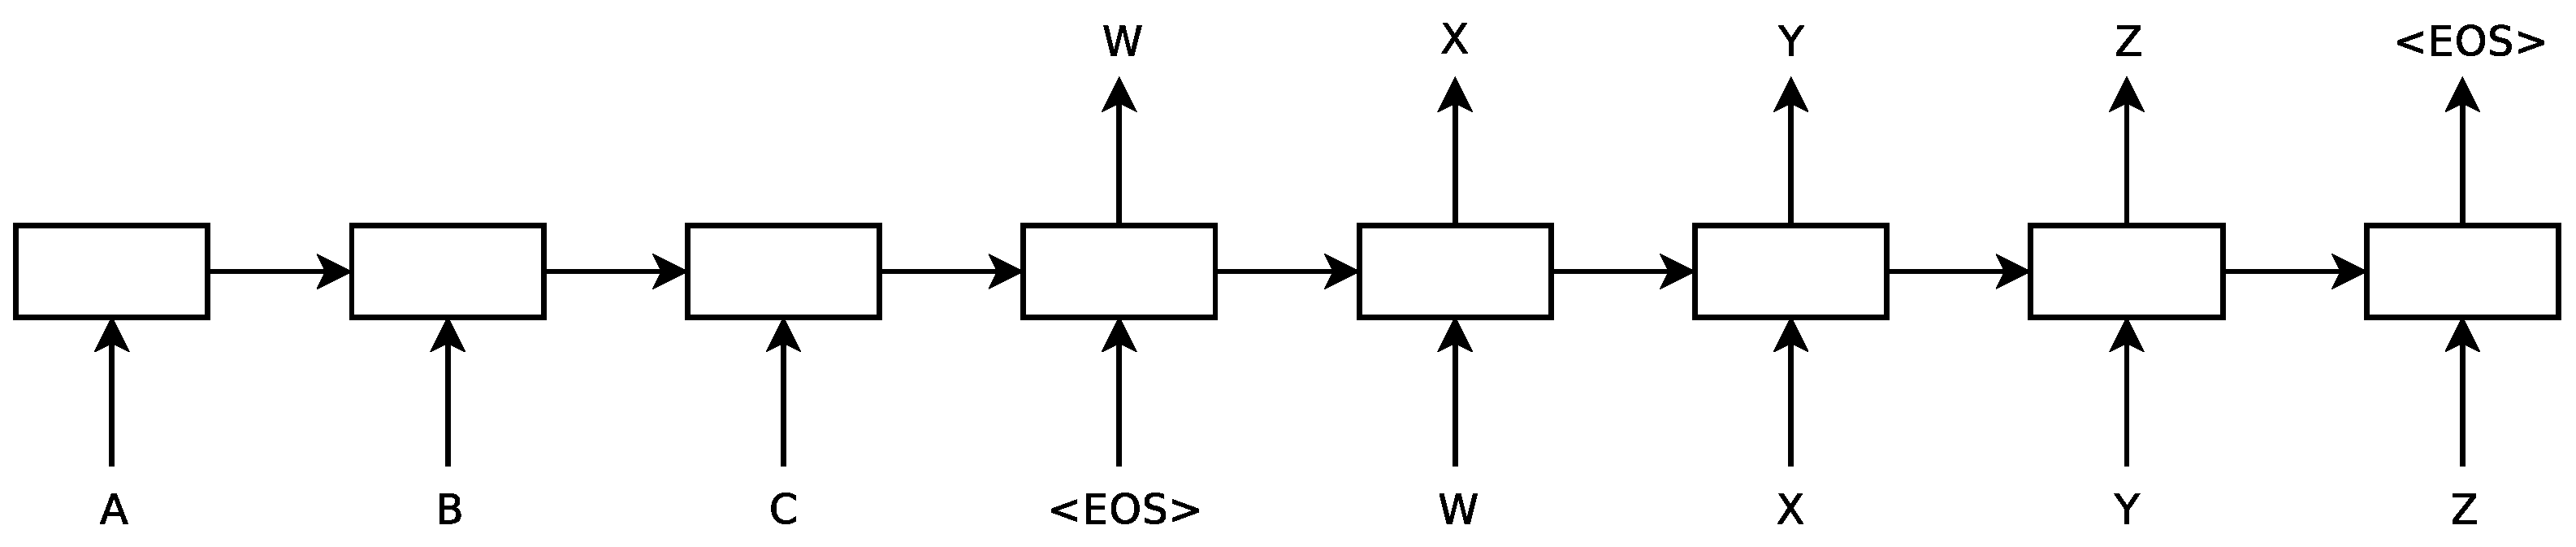
\includegraphics[width=0.9\textwidth]{./images/seq2seq/Diagram1.eps}
		\caption{\small 这个模型读入"ABC"得出"WXYZ"。模型在输出end-of-sentense token后停止预测。注意:模型是逆序读入输入句子的。}
		\label{fig:translation-model2}
	\end{figure}
	
	\section{一些细节}
	
	\begin{enumerate}
		\item 模型在找最大概率的翻译时,使用了从左到右的beam search。有趣的是在$ beam size=1 $时,模型也能得到很好的结果、$ beam size =2 $ 的性价比最高,最好的成绩在$ beam size=12 $时取到;
		\item 初始化LSTM的参数为-0.08到0.08间的均匀分布、固定学习率0.7训练5个epochs,然后每半个epoch减半,共训练7.5epochs、$ batch_size=128 $;
		\item LSTM没有发生梯度消失,但发生了梯度爆炸,为此使用了梯度裁剪;
		\item 因为句子有长有短,尽量把长度差不多的句子取在一个batch中,这样避免了算力浪费,平均加速了两倍。
	\end{enumerate}
	
	

\end{document}
